% !TEX root = trackjet_intnote.tex

The standard ATLAS event quality requirements were applied for the event selection both for the \pp\ and \PbPb\ event selection.
\begin{itemize}
\item All the sub-detector systems were required to be fully functional: all the data were required to pass the official good run list:
 \\ $\texttt{\scriptsize data15\_5TeV.periodAllYear\_DetStatus-v75-repro20-01\_DQDefects-00-02-02\_PHYS\_HeavyIonP\_All\_Good.xml}$ (2015 \pp) \\ $\texttt{\scriptsize data15\_5TeV.periodVdM\_DetStatus-v75-repro20-01\_DQDefects-00-02-02\_PHYS\_HeavyIonP\_All\_Good.xml}$ (2015, VdM \pp) \\ 
 \\ $\texttt{\scriptsize data15\_hi.periodAllYear\_DetStatus-v75-repro20-01\_DQDefects-00-02-02\_PHYS\_HeavyIonP\_All\_Good.xml } $ (2015 \pbpb).

\item All events are required to have a good reconstructed primary vertex.
\item The primary vertex must be within 150~mm from the center of ATLAS detector, as a fiducial tracking region.
 
\item Additional event cleaning to remove additional detector imperfections as described here~\cite{2015EventCleaning} is used. 
\item In \PbPb\ collisions the pileup contribution is removed using the  $\texttt{HIAnalysisTools}$ \cite{HIAnalysisTools}.  
\end{itemize}


Figures~\ref{Fig:EventCounts} presents the total number of \pp\ and \pbpb\ events, respectively, entering the analysis together with rejection power of various event quality cuts. The slightly higher fraction of empty events without primary vertex is observed in pp collisions. Some of these events are rejected by multiple cuts. ``Rejection by centrality'' indicates the number of event in HP stream that is outside the 0-80\% centrality bin.  

\begin{figure}
\centerline{
\begin{tabular}{cc}
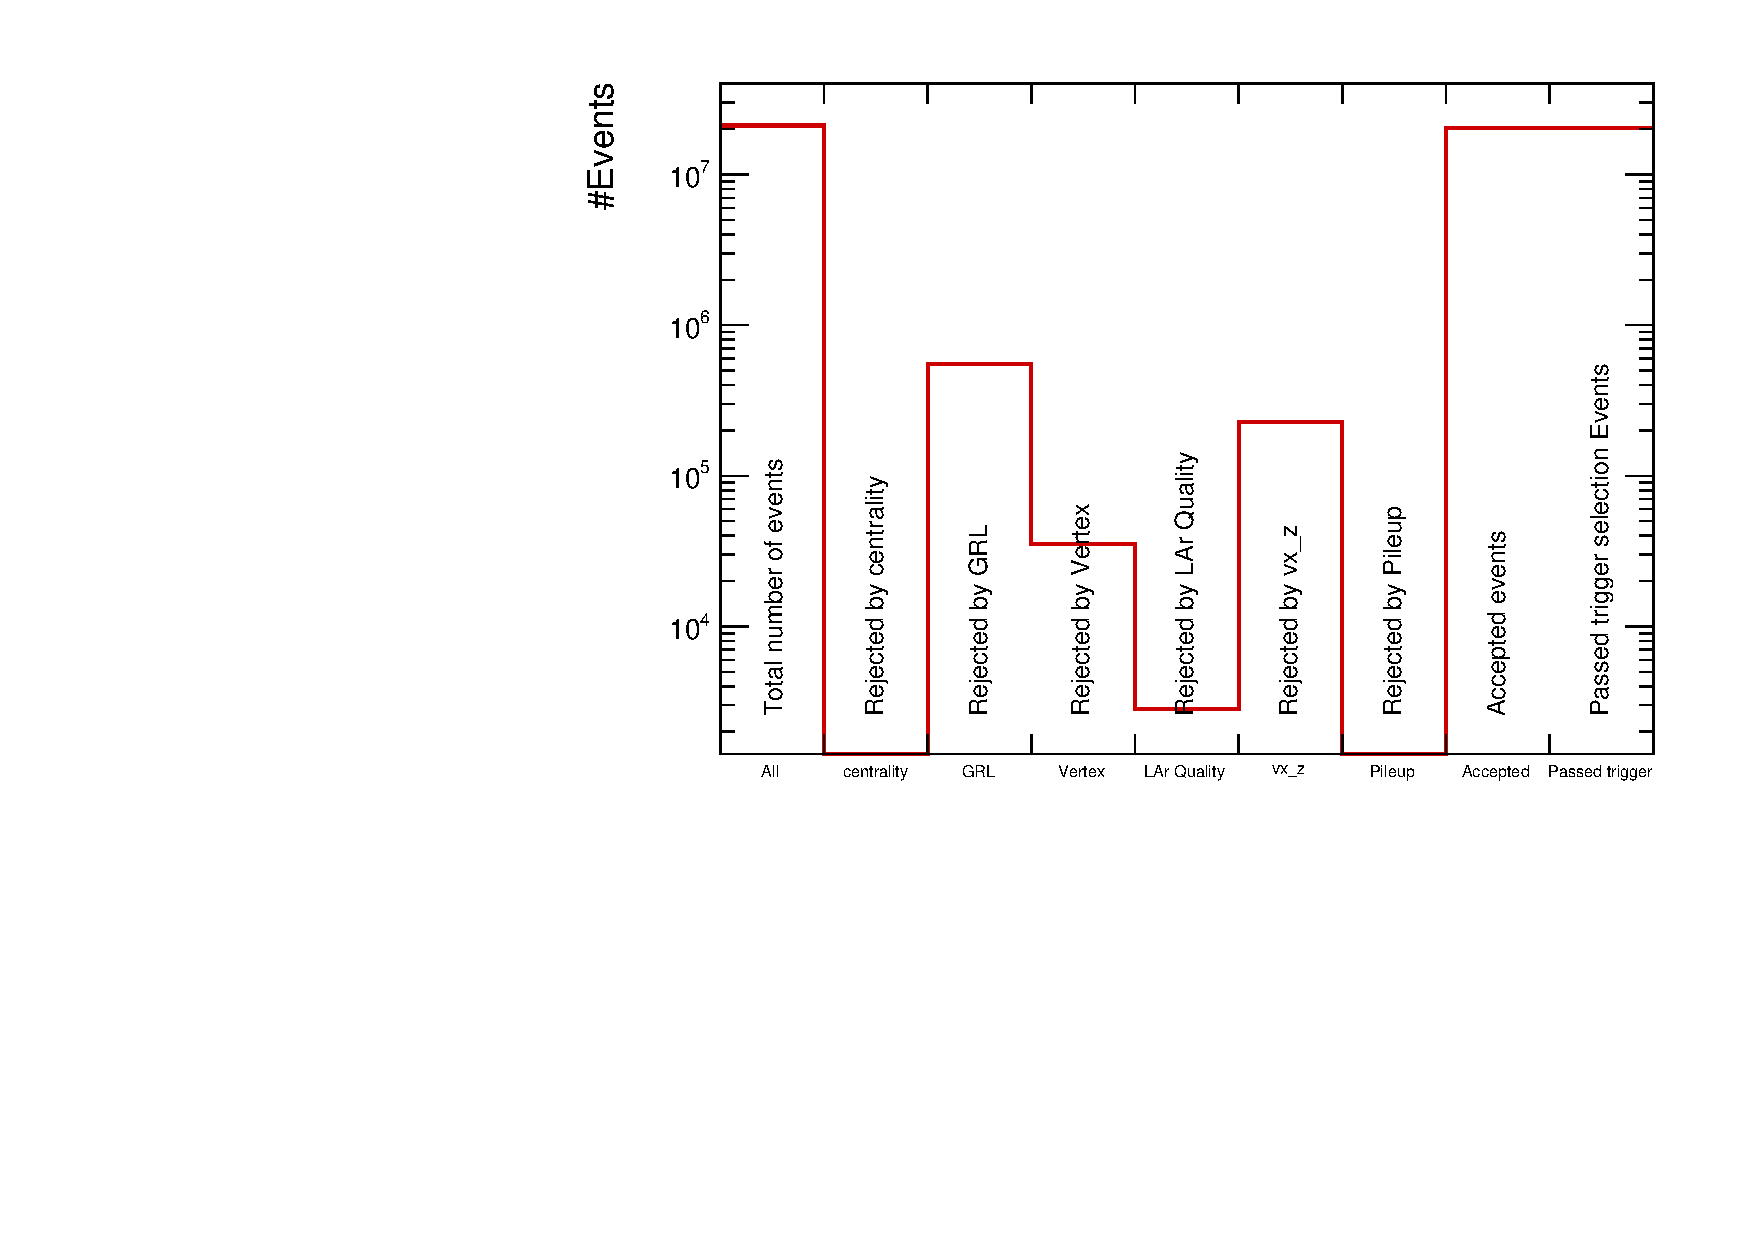
\includegraphics[width=0.45\textwidth]{figures_general/EventAccept_pp.pdf} & 
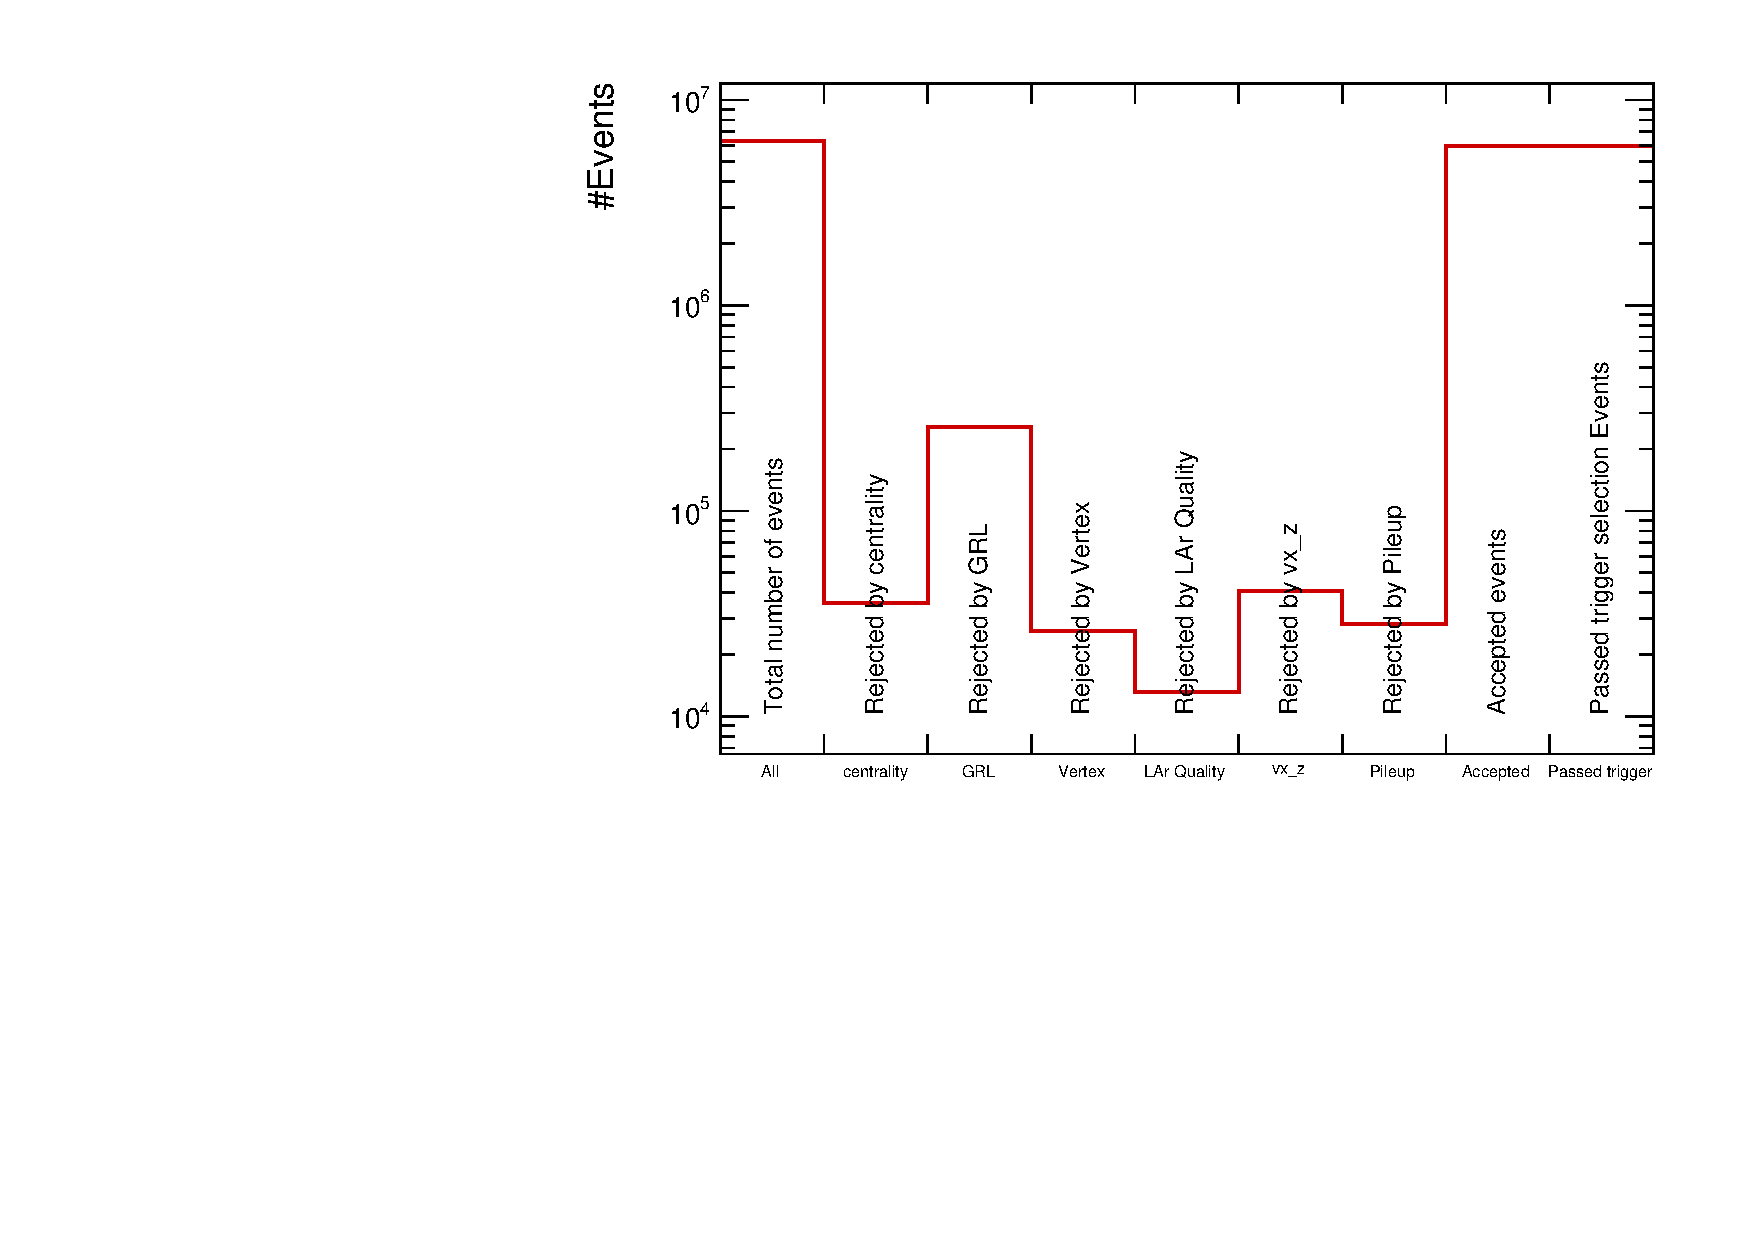
\includegraphics[width=0.45\textwidth]{figures_general/EventAccept_PbPb.pdf}
\end{tabular}}
\caption{
The number of 2015 \pp\  (left) and \PbPb\ (right) events used and rejected by various event quality cuts. }
\label{Fig:EventCounts}
\end{figure}


\subsection{Centrality Selection}
\label{sec:cent}

The centrality of the collision is a degree of the overlap of two colliding nuclei that can be quantified by the impact parameter that is the distance between the centers of the two nuclei. If they collide head on the collision is central, if they just graze each other we speak about peripheral collisions. We cannot measure the impact parameter to determine the centrality, but we can measure the overall event activity in the collision, characterized e.g. by the sum of \Et\ measured in FCal calorimeters on both sites. Central collisions have large \Et\ deposits in the FCal, peripheral have small \Et\ deposits.

In this analysis, The \ETfcal\ distribution is divided into percentiles of the total inelastic cross section for \PbPb\ collisions. The first percentile, $0-10\%$, represents the $10\%$ of collisions with the largest event activity, smallest impact parameter. The last percentile, $90-100\%$, represents the $10\%$ of collisions where there is the smallest event activity and largest impact parameter. 
Seven centrality classes have been used: 0-10\%, 10-20\%, 20-30\%, 30-40\%, 40-60\%, 60-80\%. 
The most peripheral collisions 80-100\%, are excluded due to  the small number of jets.
The centrality selections are documented in Ref.~\cite{ref:centrality}. The \PbPb\ MC is re-weighted in the way that it has the same centrality distribution as the jet triggered data sample.

\clearpage
